\title{2024 年普通高等学校招生全国统一考试（新课标 I 卷）}
\date{}
\maketitle

\section*{一、选择题}
本题共 8 小题，每小题 5 分，共 40 分. 在每小题给出的四个选项中，只有一个选项是正确的．请把正确的选项填涂在答题卡相应的位置上.

\begin{question}[points=5]
已知集合 $A = \{ x \mid -5 < x^3 < 5 \}$, $B = \{ -3, -1, 0, 2, 3 \}$, 则 $A \cap B =$
\begin{choices}
  \item $\{-1, 0\}$
  \item $\{2, 3\}$
  \item $\{-3, -1, 0\}$
  \item $\{-1, 0, 2\}$
\end{choices}
\begin{solution}
\textbf{答案：}A

\textbf{分析：}因为 $A = \{ x \mid -\sqrt[3]{5} < x < \sqrt[3]{5} \}$, $B = \{-3, -1, 0, 2, 3\}$, 且 $1 < \sqrt[3]{5} < 2$, 所以 $A \cap B = \{-1, 0\}$.
\end{solution}
\end{question}

\begin{question}[points=5]
若 $\frac{z}{z-1} = 1 + i$, 则 $z =$
\begin{choices}
  \item $-1 - i$
  \item $-1 + i$
  \item $1 - i$
  \item $1 + i$
\end{choices}
\begin{solution}
\textbf{答案：}C

\textbf{分析：}因为 $\frac{z}{z-1}=1+i$, 所以 $z=(1+i)(z-1)$，从而 $-iz=-(1+i)$，故 $z=\frac{1+i}{i}=1-i$.
\end{solution}
\end{question}

\begin{question}[points=5]
已知向量 $\vec{a} = (0,1)$, $\vec{b} = (2, x)$, 若 $\vec{b} \perp (\vec{b} - 4\vec{a})$, 则 $x =$
\begin{choices}
  \item -2
  \item -1
  \item 1
  \item 2
\end{choices}
\begin{solution}
\textbf{答案：}D

\textbf{分析：}由 $\vec{b} \perp (\vec{b} - 4\vec{a})$ 得 $\vec{b} \cdot (\vec{b} - 4\vec{a}) = 0$, 即 $4 + x^2 - 4x = 0$, 解得 $x = 2$.
\end{solution}
\end{question}

\begin{question}[points=5]
已知 $\cos(\alpha + \beta) = m$, $\tan \alpha \tan \beta = 2$, 则 $\cos(\alpha - \beta) =$
\begin{choices}
  \item $-3m$
  \item $-\frac{m}{3}$
  \item $\frac{m}{3}$
  \item $3m$
\end{choices}
\begin{solution}
\textbf{答案：}A

\textbf{分析：}由 $\cos(\alpha + \beta) = m$ 得 $\cos\alpha \cos\beta - \sin\alpha \sin\beta = m$. 又 $\tan\alpha \tan\beta = 2$, 即 $\sin\alpha \sin\beta = 2 \cos\alpha \cos\beta$. 代入得 $\cos\alpha \cos\beta - 2\cos\alpha \cos\beta = m$, 故 $\cos\alpha \cos\beta = -m$, $\sin\alpha \sin\beta = -2m$. 于是 $\cos(\alpha - \beta) = \cos\alpha \cos\beta + \sin\alpha \sin\beta = -3m$.
\end{solution}
\end{question}

\begin{question}[points=5]
已知圆柱和圆锥的底面半径相等，侧面积相等，且它们的高均为 $\sqrt{3}$, 则圆锥的体积为
\begin{choices}
  \item $2\sqrt{3}\pi$
  \item $3\sqrt{3}\pi$
  \item $6\sqrt{3}\pi$
  \item $9\sqrt{3}\pi$
\end{choices}
\begin{solution}
\textbf{答案：}B

\textbf{分析：}设圆柱的底面半径为 $r$, 则圆锥的母线长为 $\sqrt{r^2 + 3}$. 由侧面积相等得 $2\pi r \cdot \sqrt{3} = \pi r \cdot \sqrt{r^2 + 3}$, 即 $2\sqrt{3} = \sqrt{r^2 + 3}$, 解得 $r = 3$. 圆锥体积 $V = \frac{1}{3} \pi \cdot 9 \cdot \sqrt{3} = 3\sqrt{3}\pi$.
\end{solution}
\end{question}

\begin{question}[points=5]
已知函数 $f(x) = \begin{cases} -x^2 - 2ax - a, & x < 0 \\ e^x + \ln(x+1), & x \ge 0 \end{cases}$ 在 $\mathbb{R}$ 上单调递增，则 $a$ 的取值范围是
\begin{choices}
  \item $(-\infty, 0]$
  \item $[-1, 0]$
  \item $[-1, 1]$
  \item $[0, +\infty)$
\end{choices}
\begin{solution}
\textbf{答案：}B

\textbf{分析：}因为 $f(x)$ 在 $\mathbb{R}$ 上单调递增，且 $x \ge 0$ 时 $f(x) = e^x + \ln(x+1)$ 单调递增，则需满足 $\begin{cases} -\frac{-2a}{2 \times (-1)} \ge 0 \\ -a \le e^0 + \ln 1 \end{cases}$, 解得 $-1 \le a \le 0$.
\end{solution}
\end{question}

\begin{question}[points=5]
当 $x \in [0, 2\pi]$ 时，曲线 $y = \sin x$ 与 $y = 2 \sin\left(3x - \frac{\pi}{6}\right)$ 的交点个数为
\begin{choices}
  \item 3
  \item 4
  \item 6
  \item 8
\end{choices}
\begin{solution}
\textbf{答案：}C

\textbf{分析：}$y = \sin x$ 的最小正周期为 $2\pi$, $y = 2\sin(3x - \frac{\pi}{6})$ 的最小正周期为 $\frac{2\pi}{3}$, 在 $[0,2\pi]$ 上有三个周期的图象. 利用五点法画出两函数图象，可观察到有 6 个交点.
\end{solution}
\end{question}

\begin{question}[points=5]
已知函数 $f(x)$ 的定义域为 $\mathbb{R}$, $f(x) > f(x-1) + f(x-2)$, 且当 $x < 3$ 时 $f(x) = x$, 则下列结论中一定正确的是
\begin{choices}
  \item $f(10) > 100$
  \item $f(20) > 1000$
  \item $f(10) < 1000$
  \item $f(20) < 10000$
\end{choices}
\begin{solution}
\textbf{答案：}B

\textbf{分析：}由 $f(1)=1, f(2)=2$, 利用 $f(x) > f(x-1)+f(x-2)$ 递推得 $f(3)>3$, $f(4)>5$, $f(5)>8$, $f(6)>13$, $f(7)>21$, $f(8)>34$, $f(9)>55$, $f(10)>89$, $f(11)>144$, $f(12)>233$, $f(13)>377$, $f(14)>610$, $f(15)>987$, $f(16)>1597>1000$, 由此可推出 $f(20)>1000$, 故B正确.
\end{solution}
\end{question}

\section*{二、选择题}
本题共 3 小题，每小题 6 分，共 18 分. 在每小题给出的选项中，有多项符合题目要求. 全部选对得 6 分，部分选对的得部分分，选对但不全的得部分分，有选错的得 0 分.

\begin{question}[points=6]
为了解推动出口后的亩收入（单位：万元）情况，从该种植区抽取样本，得到推动出口后亩收入的样本均值 $\bar{x}=2.1$, 样本方差 $s^2=0.01$. 已知该种植区以往的亩收入 $X$ 服从正态分布 $N(1.8, 0.1^2)$, 假设推动出口后的亩收入 $Y$ 服从正态分布 $N(\bar{x}, s^2)$, 则（ ）（若随机变量 $Z$ 服从正态分布 $N(\mu, \sigma^2)$, $P(Z < \mu+\sigma) \approx 0.8413$）
\begin{choices}
  \item $P(X > 2) > 0.2$
  \item $P(X > 2) < 0.5$
  \item $P(Y > 2) > 0.5$
  \item $P(Y > 2) < 0.8$
\end{choices}
\begin{solution}
\textbf{答案：}BC

\textbf{分析：}由题 $Y \sim N(2.1, 0.1)$, 则 $P(Y > 2) = P(Y > 2.1 - 0.1) = P(Y < 2.1+0.1) \approx 0.8413 > 0.5$, 故C正确D错误. 对于 $X \sim N(1.8, 0.1)$, $P(X>2) = P(X > 1.8+2\times 0.1)$, 且 $P(X < 1.8+0.1) \approx 0.8413$, 所以 $P(X > 1.8+0.1) \approx 0.1587 < 0.2$, 于是 $P(X>2) < 0.2$, 故B正确A错误.
\end{solution}
\end{question}

\begin{question}[points=6]
设函数 $f(x) = (x-1)^2(x-4)$, 则
\begin{choices}
  \item $x=3$ 是 $f(x)$ 的极小值点
  \item 当 $0 < x < 1$ 时，$f(x) < f(x^2)$
  \item 当 $1 < x < 2$ 时，$-4 < f(2x-1) < 0$
  \item 当 $-1 < x < 0$ 时，$f(2-x) > f(x)$
\end{choices}
\begin{solution}
\textbf{答案：}ACD

\textbf{分析：}$f'(x) = 2(x-1)(x-4) + (x-1)^2 = 3(x-1)(x-3)$. 当 $x \in (1,3)$ 时 $f'(x) < 0$, 当 $x \in (-\infty,1) \cup (3,+\infty)$ 时 $f'(x) > 0$, 故 $x=3$ 是极小值点，A正确. 当 $0<x<1$ 时 $x > x^2$, 且 $f(x)$ 在 $(0,1)$ 上递增，故 $f(x) > f(x^2)$, B错误. 当 $1<x<2$ 时 $1<2x-1<3$, $f(x)$ 在 $(1,3)$ 上递减，故 $f(1) > f(2x-1) > f(3)$, 即 $-4 < f(2x-1) < 0$, C正确. 当 $-1<x<0$ 时，$f(2-x) - f(x) = (1-x)^2(-2-x) - (x-1)^2(x-4) = (x-1)^2(2-2x) > 0$, 故D正确.
\end{solution}
\end{question}

\begin{question}[points=6]
造型可以做成美丽的丝带，将其看作图中曲线 $C$ 的一部分. 已知 $C$ 过坐标原点 $O$, 且 $C$ 上的点满足横坐标大于 $-2$, 到点 $F(2,0)$ 的距离与到定直线 $x=a$ ($a<0$) 的距离之积为 4, 则

\begin{center}
  
\includegraphics[width=.36\linewidth]{question-11.png}
\end{center}
\begin{choices}
  \item $a = -2$
  \item 点 $(2\sqrt{2}, 0)$ 在 $C$ 上
  \item $C$ 在第一象限的点的纵坐标的最大值为 1
  \item 当点 $(x_0, y_0)$ 在 $C$ 上时，$y_0 \le \frac{4}{x_0+2}$
\end{choices}
\begin{solution}
\textbf{答案：}ABD

\textbf{分析：}设曲线上的动点 $P(x,y)$, 则 $x > -2$ 且 $\sqrt{(x-2)^2+y^2} \cdot |x-a| = 4$. 由曲线过原点得 $\sqrt{(0-2)^2+0^2} \cdot |0-a| = 4$, 解得 $a=-2$, A正确. 曲线方程为 $\sqrt{(x-2)^2+y^2} \cdot (x+2) = 4$. 当 $x=2\sqrt{2}, y=0$ 时，左边 $= (2\sqrt{2}-2)(2\sqrt{2}+2) = 8-4=4$, 故点在曲线上，B正确. 由曲线方程得 $y^2 = \frac{16}{(x+2)^2} - (x-2)^2$, 取 $x=3$ 得 $y^2 > 1$, 故纵坐标最大值大于1, C错误. 由 $y^2 = \frac{16}{(x+2)^2} - (x-2)^2 \le \frac{16}{(x+2)^2}$, 得 $-\frac{4}{x_0+2} \le y_0 \le \frac{4}{x_0+2}$, 故D正确.
\end{solution}
\end{question}

\section*{三、填空题}
本题共 3 小题，每小题 5 分，共 15 分.

\begin{question}[points=5]
设双曲线 $C: \frac{x^2}{a^2} - \frac{y^2}{b^2} = 1\ (a>0,b>0)$ 的左右焦点分别为 $F_1,F_2$, 过 $F_2$ 作平行于 $y$ 轴的直线交 $C$ 于 $A, B$ 两点，若 $|F_1A| = 13$, $|AB| = 10$, 则 $C$ 的离心率为
\fillin[{$\frac{3}{2}$}]
\begin{solution}
\textbf{答案：}$\frac{3}{2}$

\textbf{分析：}由题，$A,B,F_2$ 三点横坐标相等，设 $A$ 在第一象限，将 $x=c$ 代入双曲线方程得 $y = \pm \frac{b^2}{a}$, 故 $A(c,\frac{b^2}{a})$, $B(c,-\frac{b^2}{a})$, $|AB| = \frac{2b^2}{a} = 10$, 得 $\frac{b^2}{a} = 5$. 又 $|AF_1| = |AF_2| + 2a = 5 + 2a = 13$, 解得 $a=4$, $b^2=20$, $c^2 = a^2+b^2 = 36$, $c=6$, 离心率 $e = \frac{c}{a} = \frac{3}{2}$.
\end{solution}
\end{question}

\begin{question}[points=5]
若曲线 $y = e^x + x$ 在点 $(0,1)$ 处的切线也是曲线 $y = \ln(x+1) + a$ 的切线，则 $a =$
\fillin[{$\ln 2$}]
\begin{solution}
\textbf{答案：}$\ln 2$

\textbf{分析：}$y = e^x + x$ 的导数为 $y' = e^x + 1$, 在 $(0,1)$ 处切线斜率为 $2$, 切线方程为 $y = 2x + 1$. 设 $y = \ln(x+1) + a$ 的切点为 $(x_0, \ln(x_0+1)+a)$, 其导数为 $\frac{1}{x_0+1} = 2$, 解得 $x_0 = -\frac{1}{2}$, 切点为 $(-\frac{1}{2}, a + \ln\frac{1}{2})$, 切线方程为 $y = 2(x+\frac{1}{2}) + a + \ln\frac{1}{2} = 2x + 1 + a - \ln 2$. 与 $y=2x+1$ 比较得 $a - \ln 2 = 0$, 所以 $a = \ln 2$.
\end{solution}
\end{question}

\begin{question}[points=5]
甲、乙两人各有四张卡片，每张卡片上标有一个数字，甲的卡片上分别标有数字 $1,3,5,7$, 乙的卡片上分别标有数字 $2,4,6,8$. 两人进行四轮比赛，在每轮比赛中，两人各自从自己持有的卡片中随机选一张，并比较所选卡片上数字的大小，数字大的人得 1 分，数字小的人得 0 分，然后各自弃置此轮所选的卡片（弃置的卡片在此后的轮次中不能使用）. 则四轮比赛后，甲的总得分不小于 2 的概率为
\fillin[{$\frac{1}{2}$}]
\begin{solution}
\textbf{答案：}$\frac{1}{2}$

\textbf{分析：}设甲在四轮游戏中的得分分别为 $X_1,X_2,X_3,X_4$, 总得分为 $X$. 甲每轮获胜的概率均为 $\frac{3}{8}$, 故 $E(X) = \frac{3}{2}$. 记 $p_k = P(X=k)$, $k=0,1,2,3$. 甲得0分唯一对应甲出1,3,5,7对应乙出2,4,6,8, 概率 $p_0 = \frac{1}{A_4^4} = \frac{1}{24}$. 甲得3分唯一对应甲出1,3,5,7对应乙出8,2,4,6, 概率 $p_3 = \frac{1}{24}$. 由 $p_0+p_1+p_2+p_3=1$, $p_1+2p_2+3p_3 = \frac{3}{2}$, 代入得 $p_1+p_2 = \frac{11}{12}$, $p_1+2p_2 = \frac{4}{3}$, 两式相减得 $p_2 = \frac{5}{12}$, $p_3 = \frac{1}{24}$, 故 $p_2+p_3 = \frac{11}{24} + \frac{1}{24} = \frac{1}{2}$.
\end{solution}
\end{question}

\section*{四、解答题}
本题共 5 小题，共 77 分. 解答应写出文字说明、证明过程或演算步骤.

\begin{question}[points=13]
记 $\triangle ABC$ 内角 $A,B,C$ 的对边分别为 $a,b,c$, 已知 $\sin C = \sqrt{2}\cos B$, $a^2+b^2-c^2 = \sqrt{2}ab$.

(1) 求 $B$;

(2) 若 $\triangle ABC$ 的面积为 $3+\sqrt{3}$, 求 $c$.
\begin{solution}
\textbf{答案：}(1) $B = \frac{\pi}{3}$; (2) $c = 2\sqrt{2}$

\textbf{详解：}(1) 由余弦定理 $a^2+b^2-c^2 = 2ab\cos C$, 与已知比较得 $\cos C = \frac{\sqrt{2}}{2}$. 因为 $C\in(0,\pi)$, 故 $C=\frac{\pi}{4}$, $\sin C = \frac{\sqrt{2}}{2}$. 又 $\sin C = \sqrt{2}\cos B$, 得 $\cos B = \frac{1}{2}$, 所以 $B=\frac{\pi}{3}$.
(2) 由(1)得 $A = \pi - \frac{\pi}{3} - \frac{\pi}{4} = \frac{5\pi}{12}$. $\sin A = \sin\frac{5\pi}{12} = \frac{\sqrt{6}+\sqrt{2}}{4}$. 由正弦定理 $\frac{a}{\sin A} = \frac{b}{\sin B} = \frac{c}{\sin C}$, 得 $a = \frac{\sin A}{\sin C}c = \frac{\sqrt{6}+\sqrt{2}}{2}c$, $b = \frac{\sin B}{\sin C}c = \frac{\sqrt{6}}{2}c$. 三角形面积 $S = \frac{1}{2}ab\sin C = \frac{3+\sqrt{3}}{8}c^2 = 3+\sqrt{3}$, 解得 $c=2\sqrt{2}$.
\end{solution}
\end{question}

\begin{question}[points=15]
已知 $A(0,3)$ 和 $P\left(3, \frac{3}{2}\right)$ 为椭圆 $C: \frac{x^2}{a^2}+\frac{y^2}{b^2}=1\ (a>b>0)$ 上两点.

(1) 求 $C$ 的离心率;

(2) 若过 $P$ 的直线 $l$ 交 $C$ 于另一点 $B$, 且 $\triangle ABP$ 的面积为 $9$, 求 $l$ 的方程.
\begin{solution}
\textbf{答案：}(1) $\frac{1}{2}$; (2) $3x-2y-6=0$ 或 $x-2y=0$

\textbf{详解：}(1) 将 $A(0,3)$, $P(3,\frac{3}{2})$ 代入椭圆方程得 $b=3$, $a^2=12$, 故 $e = \sqrt{1-\frac{b^2}{a^2}} = \frac{1}{2}$.
(2) 法一：$k_{AP} = -\frac{1}{2}$, 直线 $AP$ 方程为 $x+2y-6=0$, $|AP| = \frac{3\sqrt{5}}{2}$. 设点 $B$ 到直线 $AP$ 的距离为 $d$, 由面积得 $d = \frac{12\sqrt{5}}{5}$. 将直线 $AP$ 平移 $\frac{12\sqrt{5}}{5}$ 单位得 $x+2y+C=0$, 由平行线距离公式得 $C=6$ 或 $C=-18$. 与椭圆联立，$C=6$ 时得 $B(0,-3)$ 或 $B(-3,-\frac{3}{2})$; $C=-18$ 时无交点. 故直线 $l$ 的斜率为 $\frac{3}{2}$ 或 $\frac{1}{2}$, 对应方程为 $3x-2y-6=0$ 或 $x-2y=0$.
\end{solution}
\end{question}

\begin{question}[points=15]
如图，四棱锥 $P-ABCD$ 中，$PA \perp$ 底面 $ABCD$, $PA=AC=2$, $BC=1$, $AB=\sqrt{3}$.

(1) 若 $AD \perp PB$, 证明：$AD \parallel$ 平面 $PBC$;

(2) 若 $AD \perp DC$, 且二面角 $A-CP-D$ 的正弦值为 $\frac{\sqrt{42}}{7}$, 求 $AD$.

\begin{center}
  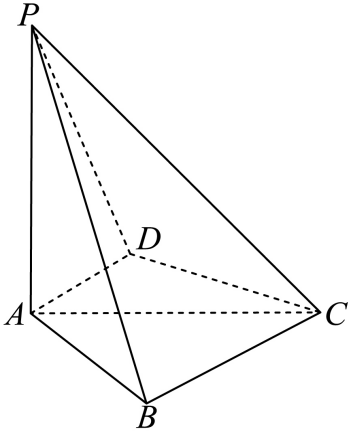
\includegraphics[width=.36\linewidth]{question-17.png}
\end{center}
\begin{solution}
\textbf{答案：}(1) 见解析; (2) $AD = \sqrt{3}$

\textbf{详解：}(1) $PA \perp$ 底面 $ABCD$, 故 $PA \perp AD$. 又 $AD \perp PB$, $PA \cap PB = P$, 所以 $AD \perp$ 平面 $PAB$, 从而 $AD \perp AB$. 由 $BC^2+AB^2 = AC^2$ 得 $BC \perp AB$, 所以 $AD // BC$. 又 $AD \not\subset$ 平面 $PBC$, $BC \subset$ 平面 $PBC$, 故 $AD //$ 平面 $PBC$.
(2) 过 $D$ 作 $DE \perp AC$ 于 $E$, 过 $E$ 作 $EF \perp CP$ 于 $F$, 连接 $DF$. 由 $PA \perp$ 底面得平面 $PAC \perp$ 平面 $ABCD$, 故 $DE \perp$ 平面 $PAC$, 则 $\angle DFE$ 为二面角 $A-CP-D$ 的平面角. $\sin\angle DFE = \frac{\sqrt{42}}{7}$, 故 $\tan\angle DFE = \sqrt{6}$. 设 $AD = x$, 则 $CD = \sqrt{4-x^2}$, 由等面积法得 $DE = \frac{x\sqrt{4-x^2}}{2}$, $CE = \frac{4-x^2}{2}$, $EF = \frac{\sqrt{2}}{2}CE = \frac{4-x^2}{2\sqrt{2}}$, 则 $\tan\angle DFE = \frac{DE}{EF} = \frac{2x\sqrt{4-x^2}}{4-x^2} \cdot \frac{1}{\sqrt{2}} = \sqrt{6}$, 解得 $x=\sqrt{3}$.
\end{solution}
\end{question}

\begin{question}[points=17]
已知函数 $f(x) = \ln\frac{x}{2-x} + ax + b(x-1)^3$.

(1) 若 $b=0$, 且 $f'(x) \ge 0$, 求 $a$ 的最小值;

(2) 证明：曲线 $y = f(x)$ 是中心对称图形;

(3) 若 $f(x) > -2$ 当且仅当 $1 < x < 2$, 求 $b$ 的取值范围.
\begin{solution}
\textbf{答案：}(1) $-2$; (2) 证明见解析; (3) $b \ge -\frac{2}{3}$

\textbf{详解：}(1) $b=0$ 时, $f(x) = \ln\frac{x}{2-x} + ax$, $x\in(0,2)$. $f'(x) = \frac{2}{x(2-x)} + a \ge 0$. 由于 $x(2-x) \le 1$, 故 $\frac{2}{x(2-x)} \ge 2$, 所以 $f'(x)_{\min} = 2 + a \ge 0$, 得 $a \ge -2$, 最小值为 $-2$.
(2) $f(x)$ 定义域为 $(0,2)$. 设 $P(m,n)$ 为图象上任意一点, 关于点 $(1,a)$ 的对称点为 $Q(2-m, 2a-n)$. 计算 $f(2-m) = \ln\frac{2-m}{m} + a(2-m) + b(1-m)^3 = -\left(\ln\frac{m}{2-m} + am + b(m-1)^3\right) + 2a = -n+2a$, 故 $Q$ 也在图象上, 因此 $y=f(x)$ 关于 $(1,a)$ 中心对称.
(3) 由 $f(x) > -2$ 当且仅当 $1 < x < 2$, 得 $f(1) = -2$, 即 $a = -2$. 此时 $f(x) > -2$ 化为 $\ln\frac{x}{2-x} + 2(1-x) + b(x-1)^3 > 0$ 在 $(1,2)$ 上恒成立. 令 $t=x-1\in(0,1)$, 则 $g(t) = \ln\frac{1+t}{1-t} - 2t + bt^3 > 0$. $g'(t) = \frac{2}{1-t^2} - 2 + 3bt^2 = \frac{t^2(3b t^2 + 2 + 3b)}{1-t^2}$.
当 $b \ge 0$ 时, $g'(t) > 0$, $g(t)$ 递增, $g(t) > g(0)=0$, 成立.
当 $-\frac{2}{3} \le b < 0$ 时, $3b t^2 + 2 + 3b \ge 2+3b \ge 0$, $g'(t) \ge 0$, 同理成立.
当 $b < -\frac{2}{3}$ 时, 存在 $t_0 \in (0,1)$ 使 $g'(t) < 0$, $g(t)$ 递减, 则 $g(t) < 0$, 不满足.
综上, $b \ge -\frac{2}{3}$.
\end{solution}
\end{question}

\begin{question}[points=17]
设 $m$ 为正整数, 数列 $a_1, a_2, \ldots, a_{4m+2}$ 是公差不为 0 的等差数列, 若从中删去两项 $a_i$ 和 $a_j$ ($i < j$) 后剩余的 $4m$ 项可被平均分为 $m$ 组, 且每组的 4 个数都能构成等差数列, 则称数列 $a_1, a_2, \ldots, a_{4m+2}$ 是 $(i,j)-$可分数列.

(1) 写出所有的 $(i,j)$, $1 \le i < j \le 6$, 使数列 $a_1, a_2, \ldots, a_6$ 是 $(i,j)-$可分数列;

(2) 当 $m \ge 3$ 时, 证明：数列 $a_1, a_2, \ldots, a_{4m+2}$ 是 $(2,13)-$可分数列;

(3) 从 $1,2,\ldots,4m+2$ 中一次任取两个数 $i$ 和 $j$ ($i < j$), 记数列 $a_1, a_2, \ldots, a_{4m+2}$ 是 $(i,j)-$可分数列的概率为 $P_m$, 证明：$P_m > \frac{1}{8}$.
\begin{solution}
\textbf{答案：}(1) $(1,2),(1,6),(5,6)$; (2) 证明见解析; (3) 证明见解析

\textbf{详解：}(1) 不妨设 $a_k = k$ (公差为1). 从 $1,2,3,4,5,6$ 中删去两项后剩余四项成等差数列, 可能的剩余组为 $\{1,2,3,4\}$, $\{2,3,4,5\}$, $\{3,4,5,6\}$, 对应删去的 $(i,j)$ 为 $(5,6)$, $(1,6)$, $(1,2)$.
(2) 设 $a_k = k$. 从 $1,2,\ldots,4m+2$ 中删去 $2$ 和 $13$ 后, 剩余数可分组为: $\{1,4,7,10\}$, $\{3,6,9,12\}$, $\{5,8,11,14\}$, 以及 $\{15,16,17,18\}$, $\{19,20,21,22\}$, $\ldots$, $\{4m-1,4m,4m+1,4m+2\}$. 共 $m$ 组, 每组成等差, 故为 $(2,13)-$可分数列.
(3) 定义 $A = \{4k+1\mid k=0,1,\ldots,m\}$, $B = \{4k+2\mid k=0,1,\ldots,m\}$. 可以证明: 若 $i\in A, j\in B$ 或 $i\in B, j\in A$, 且 $j-i\neq 3$, 则数列是 $(i,j)-$可分数列. 这样的 $(i,j)$ 共有 $(m+1)^2 - m$ 个. 总抽取方法数为 $\binom{4m+2}{2} = (2m+1)(4m+1)$. 因此 $P_m \ge \frac{(m+1)^2 - m}{(2m+1)(4m+1)} > \frac{1}{8}$.
\end{solution}
\end{question}

